\section{TRANSIT Routing}
\label{sec:transit}
The TRANSIT algorithm is based on a very simple intuition inspired from real-life navigation: when traveling
between two locations that are ``far away'' one must inevitably use some small set of edges that
are common to a great many shortest paths (highways are a natural example).
The endpoints of such edges constitute a set of so-called ``transit nodes'' for which the algorithm is named.
TRANSIT proceeds in two phases: (i) an offline precomputation phase and (ii) an online query phase.

\subsection {Precomputation}
\label{sub:precomputation}
There are two steps to TRANSIT's precomputation phase. The first step identifies transit nodes and 
the second step builds a database of exact costs. 
\newline
\textbf{Identifying Transit Nodes: } TRANSIT begins by dividing an input map into a grid of equal-sized cells~
\footnote{ This grid is distinct from the one representing the input map.}. 
To achieve this TRANSIT computes a bounding box for the entire map and divides this box
into $g \times g$ equal-size cells.  
Let $C$ denote such a cell. Further, let $I$ (Inner) and $O$ (Outer) 
be squares having $C$ in the center, as depicted in Fig. \ref{fig:example}.
The size of the squares $C$, $I$ and $O$ can be arbitrary without compromising correctness. Their exact
values however will directly impact factors such as TRANSIT's preprocessing time, storage requirements and 
online query times.
In our experiments we report results from different combinations of square sizes. We also propose some simple
heuristics for comparing between different values for these parameters.

\begin{figure}[tb]
\centering
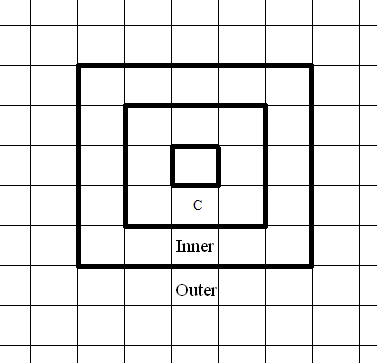
\includegraphics[height=5cm]{diagrams/transit_example3.PNG}
\caption{Example of the TRANSIT grid; also cells and inner and outer squares. }
\label{fig:example}
\end{figure}

In what follows we will compute shortest paths between nodes in $C$ and $O$ and look for
transit nodes among the endpoints of edges that cross the border of $I$.
Let $V_C$ be set of nodes as follows: for every link that has one of its endpoints inside $C$ and the other outside $C$,
$V_C$ will contain the endpoint inside $C$. Similarly, define $V_{I}$ and $V_{O}$ by considering links that cross $I$ and $O$ accordingly.
Now, the set of transit nodes for the cell $C$ is the set of nodes $v \in V_{I}$ with the property that there exists a shortest path from
some node in $V_C$ to some node in $V_{O}$ which passes through $v$. We associate every node inside $C$ with the
set of transit nodes of $C$. Next, we iterate over all cells and similarly identify transit nodes for every other cell.

\textbf{Computation and Storage of Distances: } Once we have identified all transit nodes we store, for every node on the map, the shortest distance
from this node to all its associated transit nodes.  Recall from the previous section that every
such node $v \in V$ is associated with the set of transit nodes that were found for its cell.  In
addition we also compute and store the shortest distance from each transit node to every other
transit node.  In an undirected map it is enough to compute and store costs in only one direction.

\subsection {Local Search Radius}
\label{sub:local_radius}
TRANSIT distinguishes between two types of queries: local and global.  Two nodes for which
horizontal or vertical distance (as measured in cells) is greater than some \emph{local search
radius} are considered to be "far away" and the query between them is global.  We define
local search radius to be equal to the size of the inner square $I$ plus the distance from $I$ to the
outer square $O$.
This definition guarantees that for each global query two important conditions are satisfied:
 (i) the start node $src$ and destination node $dst$ are not inside the outer squares of each other
(ii) their corresponding inner squares do not overlap. 
Both conditions are necessary to ensure the TRANSIT algorithm is correct and optimal.

\subsection{Online Query Phase}
For every global query from $src$ to $dst$ we fetch the transit nodes associated with cells containing 
$src$ and $dst$ and choose those two that will give us a minimal cost of the combined three subpaths:
$src \rightsquigarrow T_{src}$, $T_{src} \rightsquigarrow T_{dst}$, $T_{dst} \rightsquigarrow dst$.
For all local queries we apply any efficient search algorithm; A* for example.

\subsection{Shortest Path Extraction}
By performing a series of repeated distance queries TRANSIT is able to efficiently extract
actual shortest paths for any given input map. However, as path extraction is tangential to the 
current work, we omit the details of this procedure. The interested reader is instead encouraged 
to refer to the original work which contains a full description~\cite{bast06} of this method.
